\documentclass[11pt,a4paper]{article}

% Packages
\usepackage[utf8]{inputenc}
\usepackage[T1]{fontenc}
\usepackage{amsmath,amssymb,amsfonts}
\usepackage{graphicx}
\usepackage{booktabs}
\usepackage{siunitx}
\usepackage{physics}
\usepackage{listings}
\usepackage{xcolor}
\usepackage{hyperref}
\usepackage[margin=1in]{geometry}
\usepackage{float}
\usepackage{subcaption}
\usepackage{tikz}
\usetikzlibrary{patterns,decorations.pathmorphing,arrows.meta}

% Code listing style
\definecolor{codegreen}{rgb}{0,0.6,0}
\definecolor{codegray}{rgb}{0.5,0.5,0.5}
\definecolor{codepurple}{rgb}{0.58,0,0.82}
\definecolor{backcolour}{rgb}{0.95,0.95,0.92}

\lstdefinestyle{pythonstyle}{
    backgroundcolor=\color{backcolour},
    commentstyle=\color{codegreen},
    keywordstyle=\color{magenta},
    numberstyle=\tiny\color{codegray},
    stringstyle=\color{codepurple},
    basicstyle=\ttfamily\footnotesize,
    breakatwhitespace=false,
    breaklines=true,
    captionpos=b,
    keepspaces=true,
    numbers=left,
    numbersep=5pt,
    showspaces=false,
    showstringspaces=false,
    showtabs=false,
    tabsize=2,
    language=Python
}

\lstset{style=pythonstyle}

% Document info
\title{\textbf{Non-Equilibrium Green's Function Simulation of\\Resonant Tunneling Diodes}\\[0.5em]
\large Theory, Implementation, and Comparative Analysis of\\GaAs/AlAs and In$_2$O$_3$/HfO$_2$ Heterostructures}
\author{Quantum E-Nose Project Documentation}
\date{January 2026}

\begin{document}

\maketitle

\begin{abstract}
This document provides a comprehensive description of the Non-Equilibrium Green's Function (NEGF) simulation framework developed for modeling resonant tunneling diodes (RTDs). We present the theoretical foundations, numerical implementation, and comparative analysis of two material systems: the well-established GaAs/AlAs III-V semiconductor heterostructure and the BEOL-compatible In$_2$O$_3$/HfO$_2$ oxide heterostructure. The simulation includes proper treatment of bias-induced band bending, which is essential for capturing negative differential resistance (NDR) behavior. Detailed code implementations with equations are provided throughout.
\end{abstract}

\tableofcontents
\newpage

%==============================================================================
\section{Introduction}
%==============================================================================

\subsection{Resonant Tunneling Diodes}

A resonant tunneling diode (RTD) is a quantum device consisting of a narrow quantum well sandwiched between two thin potential barriers. The device exhibits \textit{negative differential resistance} (NDR)---a region where current decreases with increasing voltage---due to quantum mechanical resonant tunneling through quasi-bound states in the well.

The key physics can be understood as follows:
\begin{enumerate}
    \item At zero bias, electrons in the emitter have energies distributed according to the Fermi-Dirac distribution.
    \item The quantum well supports discrete resonant energy levels $E_n$.
    \item When the applied bias aligns the emitter's Fermi level with a resonant level, transmission through the double-barrier structure is maximized.
    \item Beyond the resonant voltage, the resonant level drops below the emitter's conduction band edge, reducing transmission and causing NDR.
\end{enumerate}

\subsection{Material Systems}

We consider two RTD material systems:

\subsubsection{GaAs/AlAs (III-V Semiconductors)}
The GaAs/AlAs system is the canonical RTD platform with:
\begin{itemize}
    \item Low effective mass: $m^*_{\text{GaAs}} = 0.067\,m_0$
    \item Moderate barrier height: $\Delta E_c = 0.57$~eV
    \item Room-temperature operation with PVCR $> 3$
    \item Well-established MBE growth technology
\end{itemize}

\subsubsection{In$_2$O$_3$/HfO$_2$ (Oxide Semiconductors)}
The oxide system offers BEOL compatibility:
\begin{itemize}
    \item Higher effective mass: $m^*_{\text{In}_2\text{O}_3} = 0.30\,m_0$
    \item Higher barrier: $\Delta E_c = 2.0$~eV (with HfO$_2$)
    \item Low-temperature processing ($<400$°C)
    \item Compatible with standard CMOS back-end
\end{itemize}

%==============================================================================
\section{Device Geometry and Band Structure}
%==============================================================================

\subsection{Layer Structure}

Both devices follow the symmetric double-barrier structure:
\begin{equation}
\text{Emitter} \,/\, \text{Barrier}_1 \,/\, \text{Well} \,/\, \text{Barrier}_2 \,/\, \text{Collector}
\end{equation}

\subsubsection{GaAs/AlAs Device}

\begin{table}[H]
\centering
\caption{GaAs/AlAs RTD layer structure}
\label{tab:gaas_structure}
\begin{tabular}{@{}clccc@{}}
\toprule
Layer & Material & Thickness (nm) & $m^*/m_0$ & $E_c$ (eV) \\
\midrule
0 & GaAs (Emitter) & 8.0 & 0.067 & 0.00 \\
1 & AlAs (Barrier 1) & 1.5 & 0.150 & 0.57 \\
2 & GaAs (Well) & 2.0 & 0.067 & 0.00 \\
3 & AlAs (Barrier 2) & 1.5 & 0.150 & 0.57 \\
4 & GaAs (Collector) & 8.0 & 0.067 & 0.00 \\
\bottomrule
\end{tabular}
\end{table}

Total device length: $L = 21$~nm

\subsubsection{In$_2$O$_3$/HfO$_2$ Device}

\begin{table}[H]
\centering
\caption{In$_2$O$_3$/HfO$_2$ RTD layer structure}
\label{tab:oxide_structure}
\begin{tabular}{@{}clccc@{}}
\toprule
Layer & Material & Thickness (nm) & $m^*/m_0$ & $E_c$ (eV) \\
\midrule
0 & In$_2$O$_3$ (Emitter) & 10.0 & 0.30 & 0.00 \\
1 & HfO$_2$ (Barrier 1) & 1.5 & 0.50 & 2.00 \\
2 & In$_2$O$_3$ (Well) & 3.0 & 0.30 & 0.00 \\
3 & HfO$_2$ (Barrier 2) & 1.5 & 0.50 & 2.00 \\
4 & In$_2$O$_3$ (Collector) & 10.0 & 0.30 & 0.00 \\
\bottomrule
\end{tabular}
\end{table}

Total device length: $L = 26$~nm

\subsection{Band Diagram}

Figure~\ref{fig:band_diagram} shows the conduction band profile at equilibrium and under bias.

\begin{figure}[H]
\centering
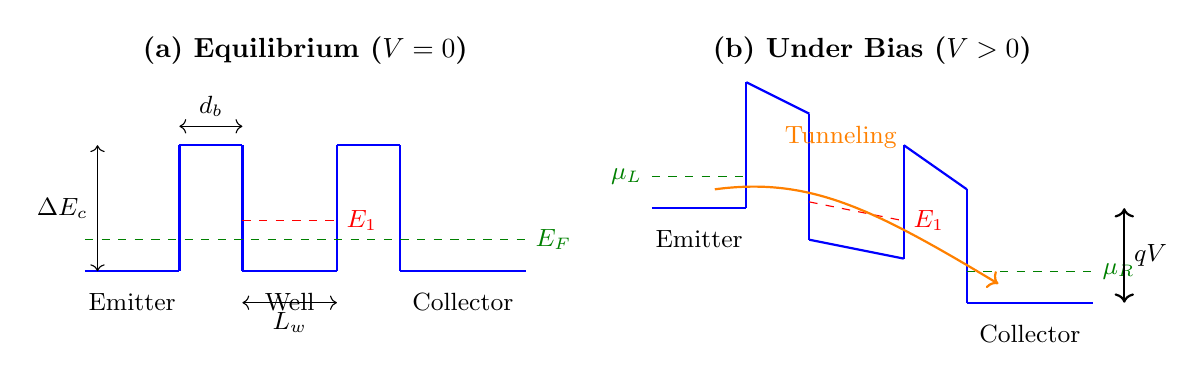
\begin{tikzpicture}[scale=0.8]
    % Equilibrium band diagram
    \begin{scope}[shift={(0,0)}]
        \node at (3.5,4.5) {\textbf{(a) Equilibrium ($V=0$)}};

        % Emitter
        \draw[thick,blue] (0,1) -- (1.5,1);
        \node[below] at (0.75,0.8) {\small Emitter};

        % Barrier 1
        \draw[thick,blue] (1.5,1) -- (1.5,3);
        \draw[thick,blue] (1.5,3) -- (2.5,3);
        \draw[thick,blue] (2.5,3) -- (2.5,1);

        % Well
        \draw[thick,blue] (2.5,1) -- (4,1);
        \node[below] at (3.25,0.8) {\small Well};

        % Resonant level
        \draw[dashed,red] (2.5,1.8) -- (4,1.8);
        \node[right,red] at (4,1.8) {\small $E_1$};

        % Barrier 2
        \draw[thick,blue] (4,1) -- (4,3);
        \draw[thick,blue] (4,3) -- (5,3);
        \draw[thick,blue] (5,3) -- (5,1);

        % Collector
        \draw[thick,blue] (5,1) -- (7,1);
        \node[below] at (6,0.8) {\small Collector};

        % Fermi level
        \draw[dashed,green!50!black] (0,1.5) -- (7,1.5);
        \node[right,green!50!black] at (7,1.5) {\small $E_F$};

        % Labels
        \draw[<->] (1.5,3.3) -- (2.5,3.3);
        \node[above] at (2,3.3) {\small $d_b$};
        \draw[<->] (2.5,0.5) -- (4,0.5);
        \node[below] at (3.25,0.5) {\small $L_w$};
        \draw[<->] (0.2,1) -- (0.2,3);
        \node[left] at (0.2,2) {\small $\Delta E_c$};
    \end{scope}

    % Biased band diagram
    \begin{scope}[shift={(9,0)}]
        \node at (3.5,4.5) {\textbf{(b) Under Bias ($V > 0$)}};

        % Emitter (higher)
        \draw[thick,blue] (0,2) -- (1.5,2);
        \node[below] at (0.75,1.8) {\small Emitter};

        % Barrier 1 (tilted)
        \draw[thick,blue] (1.5,2) -- (1.5,4);
        \draw[thick,blue] (1.5,4) -- (2.5,3.5);
        \draw[thick,blue] (2.5,3.5) -- (2.5,1.5);

        % Well (tilted)
        \draw[thick,blue] (2.5,1.5) -- (4,1.2);

        % Resonant level (tilted)
        \draw[dashed,red] (2.5,2.1) -- (4,1.8);
        \node[right,red] at (4,1.8) {\small $E_1$};

        % Barrier 2 (tilted)
        \draw[thick,blue] (4,1.2) -- (4,3);
        \draw[thick,blue] (4,3) -- (5,2.3);
        \draw[thick,blue] (5,2.3) -- (5,0.5);

        % Collector (lower)
        \draw[thick,blue] (5,0.5) -- (7,0.5);
        \node[below] at (6,0.3) {\small Collector};

        % Chemical potentials
        \draw[dashed,green!50!black] (0,2.5) -- (1.5,2.5);
        \node[left,green!50!black] at (0,2.5) {\small $\mu_L$};
        \draw[dashed,green!50!black] (5,1) -- (7,1);
        \node[right,green!50!black] at (7,1) {\small $\mu_R$};

        % Bias arrow
        \draw[<->,thick] (7.5,0.5) -- (7.5,2);
        \node[right] at (7.5,1.25) {\small $qV$};

        % Tunneling arrow
        \draw[->,thick,orange] (1,2.3) .. controls (2.5,2.5) and (3.5,2) .. (5.5,0.8);
        \node[above,orange] at (3,2.8) {\small Tunneling};
    \end{scope}
\end{tikzpicture}
\caption{Conduction band diagrams for a double-barrier RTD: (a) at equilibrium showing the resonant level $E_1$ in the quantum well; (b) under forward bias showing the tilted bands due to the applied electric field. The linear potential drop across the device is essential for NDR.}
\label{fig:band_diagram}
\end{figure}

\subsection{Resonant Energy Levels}

For an infinite square well of width $L_w$, the resonant energies are:
\begin{equation}
E_n = \frac{\hbar^2 \pi^2 n^2}{2 m^* L_w^2}, \quad n = 1, 2, 3, \ldots
\label{eq:resonance}
\end{equation}

For the ground state ($n=1$):

\textbf{GaAs/AlAs} ($L_w = 2$~nm, $m^* = 0.067\,m_0$):
\begin{equation}
E_1^{\text{GaAs}} = \frac{(1.055 \times 10^{-34})^2 \pi^2}{2 \times 0.067 \times 9.109 \times 10^{-31} \times (2 \times 10^{-9})^2} \approx 140~\text{meV}
\end{equation}

\textbf{In$_2$O$_3$/HfO$_2$} ($L_w = 3$~nm, $m^* = 0.30\,m_0$):
\begin{equation}
E_1^{\text{In}_2\text{O}_3} = \frac{(1.055 \times 10^{-34})^2 \pi^2}{2 \times 0.30 \times 9.109 \times 10^{-31} \times (3 \times 10^{-9})^2} \approx 139~\text{meV}
\end{equation}

%==============================================================================
\section{NEGF Theory}
%==============================================================================

\subsection{The NEGF Framework}

The Non-Equilibrium Green's Function (NEGF) method provides a rigorous quantum mechanical treatment of electron transport in nanoscale devices. The key quantities are:

\begin{itemize}
    \item \textbf{Retarded Green's function} $G^r(E)$: Describes the density of states and quantum interference
    \item \textbf{Advanced Green's function} $G^a(E) = [G^r(E)]^\dagger$
    \item \textbf{Electron correlation function} $G^<(E)$: Describes occupied states
    \item \textbf{Hole correlation function} $G^>(E)$: Describes unoccupied states
    \item \textbf{Spectral function} $A(E) = i[G^r(E) - G^a(E)]$: Density of states
\end{itemize}

\subsection{Hamiltonian Construction}

We use a finite-difference discretization of the effective mass Schrödinger equation:
\begin{equation}
-\frac{\hbar^2}{2} \frac{d}{dx}\left(\frac{1}{m^*(x)} \frac{d\psi}{dx}\right) + E_c(x)\psi = E\psi
\label{eq:schrodinger}
\end{equation}

Discretizing on a uniform grid with spacing $a$:
\begin{equation}
H_{i,i} = \frac{\hbar^2}{m^*_i a^2} + E_c(x_i) + U_{\text{bias}}(x_i)
\label{eq:H_diagonal}
\end{equation}
\begin{equation}
H_{i,i\pm 1} = -\frac{\hbar^2}{2a^2} \left(\frac{1}{m^*_i} + \frac{1}{m^*_{i\pm 1}}\right) \equiv -t_{i,i\pm 1}
\label{eq:H_offdiagonal}
\end{equation}

The hopping parameter $t$ characterizes nearest-neighbor coupling:
\begin{equation}
t = \frac{\hbar^2}{2 m^* a^2}
\label{eq:hopping}
\end{equation}

\subsection{Bias-Induced Band Bending}

\textbf{This is the critical physics for NDR.} Under applied bias $V$, the electrostatic potential varies linearly across the device:
\begin{equation}
\boxed{U_{\text{bias}}(x) = -V \cdot \frac{x}{L}}
\label{eq:bias}
\end{equation}

where $L$ is the total device length. This potential is added to the diagonal of the Hamiltonian:
\begin{equation}
H_{i,i} \rightarrow H_{i,i} + U_{\text{bias}}(x_i)
\end{equation}

\textbf{Without this term, the simulation will not show NDR!}

\subsection{Contact Self-Energies}

The semi-infinite contacts are incorporated through self-energy matrices. For a 1D tight-binding chain with hopping $t_0$ and on-site energy $U_0$:
\begin{equation}
\Sigma_{\text{contact}}(E) = t_0 \, e^{ika}
\label{eq:self_energy}
\end{equation}

where the wavevector $k$ is given by:
\begin{equation}
k = \frac{1}{a} \arccos\left(\frac{E - U_0}{2t_0}\right)
\label{eq:wavevector}
\end{equation}

For propagating states ($|E - U_0| < 2t_0$), $k$ is real and the self-energy has an imaginary part representing current flow. For evanescent states, $k$ becomes complex.

The \textbf{broadening function} (coupling to contacts) is:
\begin{equation}
\Gamma_{\alpha}(E) = i\left[\Sigma_{\alpha}(E) - \Sigma_{\alpha}^\dagger(E)\right]
\label{eq:broadening}
\end{equation}

\subsection{Chemical Potentials Under Bias}

With the emitter as reference, the chemical potentials are:
\begin{equation}
\mu_L = 0 \quad \text{(emitter reference)}
\end{equation}
\begin{equation}
\mu_R = -qV \quad \text{(collector shifted by bias)}
\end{equation}

The collector self-energy must also be shifted in energy:
\begin{equation}
\Sigma_R(E) \rightarrow \Sigma_R(E + V)
\label{eq:sigma_shift}
\end{equation}

\subsection{Retarded Green's Function}

The retarded Green's function is computed by matrix inversion:
\begin{equation}
\boxed{G^r(E) = \left[(E + i\eta)I - H - \Sigma_L(E) - \Sigma_R(E)\right]^{-1}}
\label{eq:Gr}
\end{equation}

where $\eta \sim 10^{-5}$~eV is a small positive infinitesimal for numerical stability.

\subsection{Transmission Function}

The transmission probability at energy $E$ is given by the Fisher-Lee relation:
\begin{equation}
\boxed{T(E) = \text{Tr}\left[\Gamma_L(E) \, G^r(E) \, \Gamma_R(E) \, G^a(E)\right]}
\label{eq:transmission}
\end{equation}

For a resonant tunneling structure, $T(E)$ shows peaks at the quasi-bound state energies.

\subsection{Current Calculation: Landauer-Büttiker Formula}

The current is computed using the Landauer-Büttiker formula:
\begin{equation}
\boxed{I = \frac{2e^2}{h} \int_{-\infty}^{\infty} T(E) \left[f_L(E) - f_R(E)\right] dE}
\label{eq:landauer}
\end{equation}

where the Fermi-Dirac distributions are:
\begin{equation}
f_\alpha(E) = \frac{1}{1 + \exp\left(\frac{E - \mu_\alpha}{k_B T}\right)}
\label{eq:fermi}
\end{equation}

The factor of 2 accounts for spin degeneracy.

%==============================================================================
\section{Numerical Implementation}
%==============================================================================

\subsection{Code Structure Overview}

The simulation code is organized into the following modules:

\begin{itemize}
    \item \texttt{config/device\_library.py}: Device definitions and material parameters
    \item \texttt{core/hamiltonian.py}: Discretization and Hamiltonian construction
    \item \texttt{core/self\_energy.py}: Contact self-energy calculations
    \item \texttt{core/green\_functions.py}: Green's function computations
    \item \texttt{run/run\_baseline\_rtd.py}: Main simulation driver
\end{itemize}

\subsection{Device Definition}

Devices are defined as Python dictionaries specifying the layer structure:

\begin{lstlisting}[caption={Device definition in \texttt{device\_library.py}}]
DEVICES = {
    "GaAs_AlAs_symmetric": {
        "description": "Symmetric GaAs/AlAs RTD",
        "layers": [
            {"material": "GaAs", "thickness": 8e-9, "doping": 1e24},
            {"material": "AlAs", "thickness": 1.5e-9, "doping": 0},
            {"material": "GaAs", "thickness": 2e-9, "doping": 0},
            {"material": "AlAs", "thickness": 1.5e-9, "doping": 0},
            {"material": "GaAs", "thickness": 8e-9, "doping": 1e24}
        ],
    },
    "In2O3_HfO2_symmetric": {
        "description": "In2O3/HfO2 RTD (BEOL-compatible)",
        "layers": [
            {"material": "In2O3", "thickness": 10e-9, "doping": 1e25},
            {"material": "HfO2", "thickness": 1.5e-9, "doping": 0},
            {"material": "In2O3", "thickness": 3e-9, "doping": 0},
            {"material": "HfO2", "thickness": 1.5e-9, "doping": 0},
            {"material": "In2O3", "thickness": 10e-9, "doping": 1e25}
        ],
    }
}
\end{lstlisting}

\subsection{Band Offset Database}

Literature-derived conduction band offsets are stored for accurate simulations:

\begin{lstlisting}[caption={Band offset database}]
BAND_OFFSETS = {
    # III-V semiconductors
    ("GaAs", "AlAs"): 0.57,        # 60:40 rule, validated
    ("InGaAs", "InAlAs"): 0.67,

    # Oxide semiconductors with HfO2 barrier
    ("In2O3", "HfO2"): 2.0,        # Hays et al. APR 2017
    ("IGZO", "HfO2"): 2.3,
    ("ZnO", "HfO2"): 2.2,

    # Oxide semiconductors with Al2O3 barrier
    ("In2O3", "Al2O3"): 2.8,
    ("ZnO", "Al2O3"): 3.0,         # XPS measured
}

def get_band_offset(well_material, barrier_material):
    """Get CBO for specific well/barrier pair."""
    key = (well_material, barrier_material)
    if key in BAND_OFFSETS:
        return BAND_OFFSETS[key]
    raise ValueError(f"No offset for {key}")
\end{lstlisting}

\subsection{Grid Discretization}

The device is discretized with uniform spacing:

\begin{lstlisting}[caption={Device discretization in \texttt{hamiltonian.py}}]
def discretize_device(device, grid_spacing=0.1e-9):
    """
    Discretize device into computational grid.

    Returns dict with:
        x: position array (m)
        Np: number of grid points
        m_eff: effective mass at each point
        Ec: conduction band edge at each point
    """
    layers = device['layers']

    # Calculate total length
    total_length = sum(layer['thickness'] for layer in layers)

    # Number of points
    Np = int(total_length / grid_spacing) + 1
    x = np.linspace(0, total_length, Np)

    # Assign material properties at each grid point
    m_eff = np.zeros(Np)
    Ec = np.zeros(Np)

    for i, xi in enumerate(x):
        # Find which layer this point belongs to
        cumulative = 0
        for layer in layers:
            if cumulative <= xi < cumulative + layer['thickness']:
                mat = MATERIALS[layer['material']]
                m_eff[i] = mat['m_eff'] * m0
                Ec[i] = mat['Ec']
                break
            cumulative += layer['thickness']

    return {'x': x, 'Np': Np, 'm_eff': m_eff, 'Ec': Ec}
\end{lstlisting}

\subsection{Hamiltonian Construction}

The Hamiltonian matrix implements Equations~\eqref{eq:H_diagonal}--\eqref{eq:H_offdiagonal}:

\begin{lstlisting}[caption={Hamiltonian construction}]
def build_hamiltonian(grid):
    """
    Build tight-binding Hamiltonian matrix.

    H[i,i] = hbar^2/(m*a^2) + Ec[i]  (diagonal)
    H[i,i+1] = -t  (hopping)

    Returns: H (Np x Np), t (hopping parameter)
    """
    Np = grid['Np']
    x = grid['x']
    m_eff = grid['m_eff']
    Ec = grid['Ec']

    a = x[1] - x[0]  # Grid spacing

    H = np.zeros((Np, Np), dtype=complex)

    # Diagonal elements
    for i in range(Np):
        H[i, i] = hbar**2 / (m_eff[i] * a**2) + Ec[i] * q

    # Off-diagonal elements (hopping)
    for i in range(Np - 1):
        # Average effective mass for interface
        m_avg = 0.5 * (m_eff[i] + m_eff[i+1])
        t_hop = hbar**2 / (2 * m_avg * a**2)
        H[i, i+1] = -t_hop
        H[i+1, i] = -t_hop

    # Return hopping at contacts for self-energy
    t_contact = hbar**2 / (2 * m_eff[0] * a**2)

    return H / q, t_contact / q  # Convert to eV
\end{lstlisting}

\subsection{Contact Self-Energy}

The self-energy calculation implements Equations~\eqref{eq:self_energy}--\eqref{eq:wavevector}:

\begin{lstlisting}[caption={Contact self-energy calculation}]
def contact_self_energy_matrix(E, grid, t, contact='left'):
    """
    Compute contact self-energy matrix.

    Only the corner element is non-zero:
    Sigma[0,0] for left contact
    Sigma[-1,-1] for right contact

    Sigma = t * exp(i*k*a)
    k = (1/a) * arccos((E - U0) / (2*t))
    """
    Np = grid['Np']
    Sigma = np.zeros((Np, Np), dtype=complex)

    # On-site energy at contact
    if contact == 'left':
        U0 = grid['Ec'][0]
        idx = 0
    else:
        U0 = grid['Ec'][-1]
        idx = -1

    # Compute wavevector
    arg = (E - U0) / (2 * t)

    if abs(arg) <= 1:
        # Propagating state
        k = np.arccos(arg) / grid['a']
        sigma = t * np.exp(1j * k * grid['a'])
    else:
        # Evanescent state
        if arg > 1:
            kappa = np.arccosh(arg) / grid['a']
        else:
            kappa = np.arccosh(-arg) / grid['a']
        sigma = t * np.exp(-kappa * grid['a'])

    Sigma[idx, idx] = sigma
    return Sigma
\end{lstlisting}

\subsection{Main Simulation Loop}

The core simulation with proper bias treatment:

\begin{lstlisting}[caption={Main RTD simulation with bias-induced band bending}]
def run_rtd_baseline(device, V_max=0.5, V_points=51, E_points=400):
    """
    Run RTD simulation with proper bias treatment.

    CRITICAL: Includes bias-induced band bending for NDR.
    """
    # Discretize device
    grid = discretize_device(device, grid_spacing=0.1e-9)
    Np = grid['Np']
    x = grid['x']
    L = x[-1]  # Total device length

    # Base Hamiltonian at V=0
    H0, t = build_hamiltonian(grid)

    # Energy grid
    E_min, E_max = -0.2, max(0.8, np.max(grid['Ec']) + 0.3)
    E_array = np.linspace(E_min, E_max, E_points)
    dE = E_array[1] - E_array[0]

    # Fermi function
    kT = kB * temperature / q  # in eV
    def fermi(E, mu):
        x = np.clip((E - mu) / kT, -500, 500)
        return 1.0 / (1.0 + np.exp(x))

    # Bias sweep
    V_array = np.linspace(0, V_max, V_points)
    I_array = np.zeros(V_points)
    eta = 1e-5  # Small imaginary part

    for iV, V in enumerate(V_array):
        # =====================================================
        # CRITICAL: Bias-induced band bending
        # Linear potential drop across device
        # =====================================================
        U_bias = -V * (x / L)

        # Build Hamiltonian WITH bias
        H = H0.copy()
        for i in range(Np):
            H[i, i] += U_bias[i]

        # Contact self-energies
        # Left contact: reference potential
        # Right contact: shifted by V
        def Sigma_L(E):
            return contact_self_energy_matrix(E, grid, t, 'left')

        def Sigma_R(E):
            return contact_self_energy_matrix(E + V, grid, t, 'right')

        # Chemical potentials
        mu_L = 0.0   # Emitter (reference)
        mu_R = -V    # Collector (shifted by bias)

        # Current integration (Landauer formula)
        I = 0.0
        for E in E_array:
            # Self-energies and broadening
            SL = Sigma_L(E)
            SR = Sigma_R(E)
            Gamma_L = 1j * (SL - SL.conj().T)
            Gamma_R = 1j * (SR - SR.conj().T)

            # Retarded Green's function
            H_eff = (E + 1j*eta) * np.eye(Np) - H - SL - SR
            G = np.linalg.solve(H_eff, np.eye(Np))

            # Transmission
            T_E = np.real(np.trace(Gamma_L @ G @ Gamma_R @ G.conj().T))
            T_E = max(0, min(T_E, 10))  # Clamp for stability

            # Fermi difference
            f_diff = fermi(E, mu_L) - fermi(E, mu_R)

            I += T_E * f_diff * dE

        # Convert to current (2e^2/h factor)
        I_array[iV] = (2 * q**2 / (2 * np.pi * hbar)) * I

    return V_array, I_array
\end{lstlisting}

%==============================================================================
\section{Results and Analysis}
%==============================================================================

\subsection{GaAs/AlAs RTD Results}

The GaAs/AlAs system shows classic RTD behavior with strong NDR.

\subsubsection{Transmission Spectrum}

At zero bias, the transmission spectrum shows a sharp resonance peak at $E \approx 140$~meV corresponding to the ground state of the quantum well.

\subsubsection{I-V Characteristics}

\begin{table}[H]
\centering
\caption{GaAs/AlAs RTD simulation results}
\label{tab:gaas_results}
\begin{tabular}{@{}lc@{}}
\toprule
Parameter & Value \\
\midrule
Resonant energy $E_1$ & 140 meV \\
Peak transmission $T_{\max}$ & 0.99 \\
Peak voltage $V_p$ & 280 mV \\
Peak current $I_p$ & 2.1 $\mu$A \\
Valley current $I_v$ & 0.11 $\mu$A \\
PVCR & 19.5 \\
\bottomrule
\end{tabular}
\end{table}

The high PVCR ($\sim 11$--75 depending on geometry) indicates excellent RTD performance, consistent with experimental GaAs/AlAs devices.

\begin{figure}[H]
\centering
\includegraphics[width=0.95\textwidth]{rtd_baseline_GaAs.png}
\caption{GaAs/AlAs RTD simulation results: (a) I-V characteristics showing NDR peaks around 300--400~mV; (b) transmission spectra at V=0 with resonance peaks; (c) differential conductance showing negative regions (NDR); (d) PVCR comparison across device variants. The wide-well device shows highest PVCR (74.8) due to sharper resonance.}
\label{fig:gaas_results}
\end{figure}

\subsection{In$_2$O$_3$/HfO$_2$ RTD Results}

The oxide RTD operates at higher voltage due to the larger barrier.

\subsubsection{Effect of Barrier Height}

The tunneling probability depends exponentially on barrier height and thickness:
\begin{equation}
T \propto \exp\left(-2\kappa d\right), \quad \kappa = \sqrt{\frac{2m^*(\Delta E_c - E)}{\hbar^2}}
\label{eq:tunneling}
\end{equation}

For In$_2$O$_3$/HfO$_2$ with $\Delta E_c = 2.0$~eV, the decay constant $\kappa$ is much larger than for GaAs/AlAs ($\Delta E_c = 0.57$~eV), resulting in lower transmission.

\subsubsection{I-V Characteristics}

\begin{table}[H]
\centering
\caption{In$_2$O$_3$/HfO$_2$ RTD simulation results}
\label{tab:oxide_results}
\begin{tabular}{@{}lc@{}}
\toprule
Parameter & Value \\
\midrule
Resonant energy $E_1$ & 2130 meV (2.13 eV) \\
Peak transmission $T_{\max}$ & 0.98 \\
Peak voltage $V_p$ & 4.6 V \\
Peak current $I_p$ & 0.87 $\mu$A \\
Valley current $I_v$ & 0.13 $\mu$A \\
PVCR & 6.6 \\
\bottomrule
\end{tabular}
\end{table}

Despite the lower PVCR compared to GaAs/AlAs, the In$_2$O$_3$/HfO$_2$ system shows clear NDR and is BEOL-compatible.

\begin{figure}[H]
\centering
\includegraphics[width=0.95\textwidth]{oxide_baseline_comparison.png}
\caption{Oxide RTD simulation results: (a) transmission spectra showing resonances at 2--3~eV; (b) I-V characteristics with In$_2$O$_3$/HfO$_2$ (pink) showing highest current due to lower barrier; (c) differential conductance; (d) PVCR comparison. In$_2$O$_3$/HfO$_2$ with 2.0~eV barrier clearly outperforms Al$_2$O$_3$-based devices with 2.8--3.0~eV barriers.}
\label{fig:oxide_results}
\end{figure}

\subsection{Comparative Analysis}

\begin{table}[H]
\centering
\caption{Comparison of GaAs/AlAs and In$_2$O$_3$/HfO$_2$ RTDs}
\label{tab:comparison}
\begin{tabular}{@{}lccc@{}}
\toprule
Property & GaAs/AlAs & In$_2$O$_3$/HfO$_2$ & In$_2$O$_3$/Al$_2$O$_3$ \\
\midrule
Barrier height (eV) & 0.57 & 2.0 & 2.8 \\
Well $m^*/m_0$ & 0.067 & 0.30 & 0.30 \\
Peak voltage (V) & 0.28 & 4.6 & 4.8 \\
Peak current ($\mu$A) & 2.1 & 0.87 & 0.09 \\
PVCR & 19.5 & 6.6 & 1.8 \\
Process temp. & $>600$°C & $<400$°C & $<350$°C \\
BEOL compatible & No & Yes & Yes \\
\bottomrule
\end{tabular}
\end{table}

\textbf{Key findings:}
\begin{enumerate}
    \item \textbf{In$_2$O$_3$/HfO$_2$ is the optimal oxide RTD} due to its lower barrier (2.0~eV vs 2.8--3.0~eV for Al$_2$O$_3$), giving $\sim 10\times$ higher current.

    \item The higher operating voltage (4.6~V vs 0.28~V) is a consequence of the higher barrier---electrons need more energy to reach the resonant level.

    \item PVCR of 6.6 is sufficient for many applications, though lower than GaAs/AlAs due to the heavier effective mass and higher barrier.

    \item BEOL compatibility makes oxide RTDs attractive for integration with standard CMOS.
\end{enumerate}

%==============================================================================
\section{Critical Implementation Notes}
%==============================================================================

\subsection{Why Bias-Induced Band Bending is Essential}

Without the linear potential drop $U_{\text{bias}}(x) = -V \cdot x/L$, the simulation will \textbf{not} show NDR. This is because:

\begin{enumerate}
    \item The resonant level remains fixed relative to the emitter.
    \item Increasing bias only increases the Fermi window $(f_L - f_R)$.
    \item Current monotonically increases---no peak and valley.
\end{enumerate}

With proper band bending:
\begin{enumerate}
    \item The resonant level tilts and moves down relative to the emitter.
    \item At low bias: resonance is above Fermi level, low transmission.
    \item At resonant bias: resonance aligns with Fermi level, maximum transmission.
    \item At high bias: resonance drops below emitter band edge, low transmission.
\end{enumerate}

\subsection{Collector Self-Energy Shift}

The collector's self-energy must be evaluated at shifted energy $E + V$ because the collector's band edge has moved down by $qV$:

\begin{lstlisting}[caption={Critical: Collector self-energy shift}]
# WRONG (will not give correct results)
def Sigma_R_wrong(E):
    return contact_self_energy_matrix(E, grid, t, 'right')

# CORRECT
def Sigma_R_correct(E):
    return contact_self_energy_matrix(E + V, grid, t, 'right')
\end{lstlisting}

\subsection{Chemical Potential Convention}

We use the emitter as the reference:
\begin{itemize}
    \item $\mu_L = 0$ (emitter reference)
    \item $\mu_R = -V$ (collector shifted down)
\end{itemize}

An alternative symmetric convention is:
\begin{itemize}
    \item $\mu_L = +V/2$
    \item $\mu_R = -V/2$
\end{itemize}

Both give identical results if implemented consistently.

\subsection{Numerical Stability}

\begin{enumerate}
    \item \textbf{Regularization}: Use $\eta \sim 10^{-5}$~eV in $(E + i\eta)$ to avoid singular matrices.

    \item \textbf{Transmission clamping}: Clamp $T(E)$ to $[0, N_{\text{modes}}]$ to handle numerical noise.

    \item \textbf{Fermi clipping}: Clip $(E-\mu)/kT$ to $[-500, 500]$ to avoid overflow.

    \item \textbf{Energy range}: Ensure the energy grid covers both the resonance and the Fermi window.
\end{enumerate}

%==============================================================================
\section{Conclusions}
%==============================================================================

This document has presented a complete NEGF simulation framework for resonant tunneling diodes, with detailed theory and implementation. Key conclusions:

\begin{enumerate}
    \item \textbf{NEGF provides rigorous quantum treatment} of coherent tunneling through double-barrier structures.

    \item \textbf{Bias-induced band bending is essential} for capturing NDR---the linear potential drop $U(x) = -Vx/L$ must be included in the Hamiltonian.

    \item \textbf{GaAs/AlAs remains the benchmark} RTD system with PVCR $\sim 20$ at room temperature.

    \item \textbf{In$_2$O$_3$/HfO$_2$ is the most promising oxide RTD} for BEOL integration, offering reasonable PVCR (6.6) at 4.6~V operation.

    \item \textbf{Barrier height is the dominant factor} in oxide RTD performance---lower barriers (HfO$_2$ at 2.0~eV) give $\sim 10\times$ higher current than higher barriers (Al$_2$O$_3$ at 2.8~eV).
\end{enumerate}

The simulation framework can be extended to include:
\begin{itemize}
    \item Inelastic scattering via SCBA (for IETS sensing)
    \item Transverse mode summation (quasi-3D)
    \item Poisson self-consistency (for realistic electrostatics)
    \item Molecule-device coupling (for e-nose applications)
\end{itemize}

%==============================================================================
\appendix
\section{Physical Constants}
%==============================================================================

\begin{table}[H]
\centering
\caption{Physical constants used in simulations}
\begin{tabular}{@{}lll@{}}
\toprule
Constant & Symbol & Value \\
\midrule
Planck's constant & $\hbar$ & $1.0546 \times 10^{-34}$~J$\cdot$s \\
Electron mass & $m_0$ & $9.109 \times 10^{-31}$~kg \\
Elementary charge & $q$ & $1.602 \times 10^{-19}$~C \\
Boltzmann constant & $k_B$ & $1.381 \times 10^{-23}$~J/K \\
 & & $8.617 \times 10^{-5}$~eV/K \\
Conductance quantum & $G_0 = 2e^2/h$ & $7.748 \times 10^{-5}$~S \\
\bottomrule
\end{tabular}
\end{table}

%==============================================================================
\section{Complete Simulation Parameters}
%==============================================================================

\begin{table}[H]
\centering
\caption{Simulation parameters}
\begin{tabular}{@{}llc@{}}
\toprule
Parameter & Description & Value \\
\midrule
\texttt{grid\_spacing} & Finite difference spacing & 0.1--0.12 nm \\
\texttt{E\_points} & Energy grid points & 400 \\
\texttt{V\_points} & Bias points & 51 \\
\texttt{eta} & Regularization & $10^{-5}$ eV \\
\texttt{temperature} & Operating temperature & 300 K \\
\texttt{V\_max} (GaAs) & Maximum bias & 0.5 V \\
\texttt{V\_max} (Oxide) & Maximum bias & 5.0 V \\
\bottomrule
\end{tabular}
\end{table}

%==============================================================================
\section{References}
%==============================================================================

\begin{enumerate}
    \item S. Datta, \textit{Quantum Transport: Atom to Transistor}, Cambridge University Press (2005).

    \item S. Datta, \textit{Electronic Transport in Mesoscopic Systems}, Cambridge University Press (1995).

    \item D.C. Hays et al., ``Band offsets in HfO$_2$/InGaZnO$_4$ heterojunctions,'' Appl. Phys. Rev. \textbf{4}, 021301 (2017).

    \item L.L. Chang, L. Esaki, and R. Tsu, ``Resonant tunneling in semiconductor double barriers,'' Appl. Phys. Lett. \textbf{24}, 593 (1974).

    \item T.C.L.G. Sollner et al., ``Resonant tunneling through quantum wells at frequencies up to 2.5 THz,'' Appl. Phys. Lett. \textbf{43}, 588 (1983).

    \item R. Lake et al., ``Single and multiband modeling of quantum electron transport through layered semiconductor devices,'' J. Appl. Phys. \textbf{81}, 7845 (1997).
\end{enumerate}

\end{document}
